\section{Design Requirements} \label{sec:hardware}\label{sec:design_requirements}



In designing and implementing CALIS the following constraints have to be taken into account and The system includes several safety features to ensure safe deployment and retrieval of the source without affecting the neutron veto detector:
\begin{description}
%organ pipe already introduced?
%pig? calibration device, source deployment mechanism.
\item The calibration device (the so called "pig") is deployed in the \lsv and thereby gets immersed in the liquid scintillator. The liquid scintillator however may not get in touch with oxygen or water, and therefore the apparatus is completely sealed during deployments to maintain the liquid scintillator under a nitrogen blanket 100 \% of the time. Small level and pressure changes as introduced by the pig during insertion into the LS can be tolerated by the \lsv\ and are taken care of by the slow control system.
%tested for helium leak tightness

\item The source may not get in contact with the liquid scintillator. It is therefore sealed during the deployment in a dedicated source holder. In order to exchange sources the source arm and source holder has to be extracted from the pig into CRH and thereby comes in contact with normal air, containing oxygen and traces of water. After insertion a flush \& purge cycle is used to reduce, as known from glove boxes. No glove box present. Much more compact design.
% no glove box



%precise: center of the \tpc\ ... m below the gate valve.
\item The center of the \tpc\ is about 7 m below CRH and the organ pipes are about 80 cm off axis. In order to deploy a radioactive source next to the cryostat an arm has to be part of the so called pig. At the same time the deployment precision has to be at the $\pm 1$ cm level both in Z and XY.
\item[material and cleanliness] 
All materials that come in contact with the scintillator veto are made of stainless steel and teflon except for the sealing o-rings which are made out of viton.  All three materials (stainless steel, teflon, and viton) are certified materials for contact with TMB and liquid scintillator in the neutron veto.

Before assembly in CRH, each component of CALIS, the ones introduced into the scintillator as well as those in the clean room CRH, have been subjected to the usual (?!) cleaning procedure, approved for interaction with the scintillator.

\end{description}

\subsection{Hardware}

The overall device consists of three main assemblies: the lower assembly, upper assembly, and the source deployment mechanism. Fig \ref{fig:wholeAssembly_insideDetectors} shows the layout of the system as installed CRH and deployed in Liquid Scintillator Veto (LSV). Fig. \ref{fig:CALISDimensions3} shows the details of the full device with all dimensions included. The lower assembly (Section \ref{The Lower Assembly}) is attached to the top of the gate valve (that closes the organ pipe in CRH), visible at the bottom of the Fig.\ref{fig:CALISDimensions3} and portruding to the left. On the top of the lower  assembly is a view port  (depicted in blue) and an access point for accessing the arm and exchanging sources. The structure shaped like two joint cones below the viewport guides the system smoothly down the organ pipe. Source capsule is visible inside the blue viewport. Circular gear above the viewport allows the rotation of the source arm to horizontal position as shown. The second conical cap above the rotation gear mechanism contains a cylindrical weight to minimize any lateral motion or oscillations during deployment and articulation and dearticulation especially. It also ensures smooth motion of the CALIS III into the organ pipe and back to the top park position. Fig \ref{fig:sourcePod_arrows} shows the photo of these parts as assembled. Inside the upper assembly (Section \ref{The Upper Assembly}) that attaches to the lower assembly are the two spools (shown in profile) used to wind and unwind two cables that hold the deployment mechanism simultaneously. The spools are attached to a single shaft rotated by the stepper motor drive shown at the top right side of the upper assembly. Small circular object located at the top left of the upper assembly is the manual handle for source arm articulation to horizontal position and back to vertical position during deployments.  The drive mechanism is controlled via a LabVIEW interface (Section \ref{LabView}).  The third assembly of the device that contains the source deployment mechanism is called "the pig", Section \ref{The Pig}. It encompases the arm, the source container (located at the end of the arm), and two conical shells (mentioned above) for the smooth transportation of the source  (again see Fig \ref{fig:sourcePod_arrows} for details). The pig is stored in the upper assembly, with the source arm in view, through the view port of the lower assembly. This allows the gate valve to remain closed except during calibration of the detector. During deployments the whole pig is lowered into the detector. 

\begin{figure}[htbp]
 \centering
 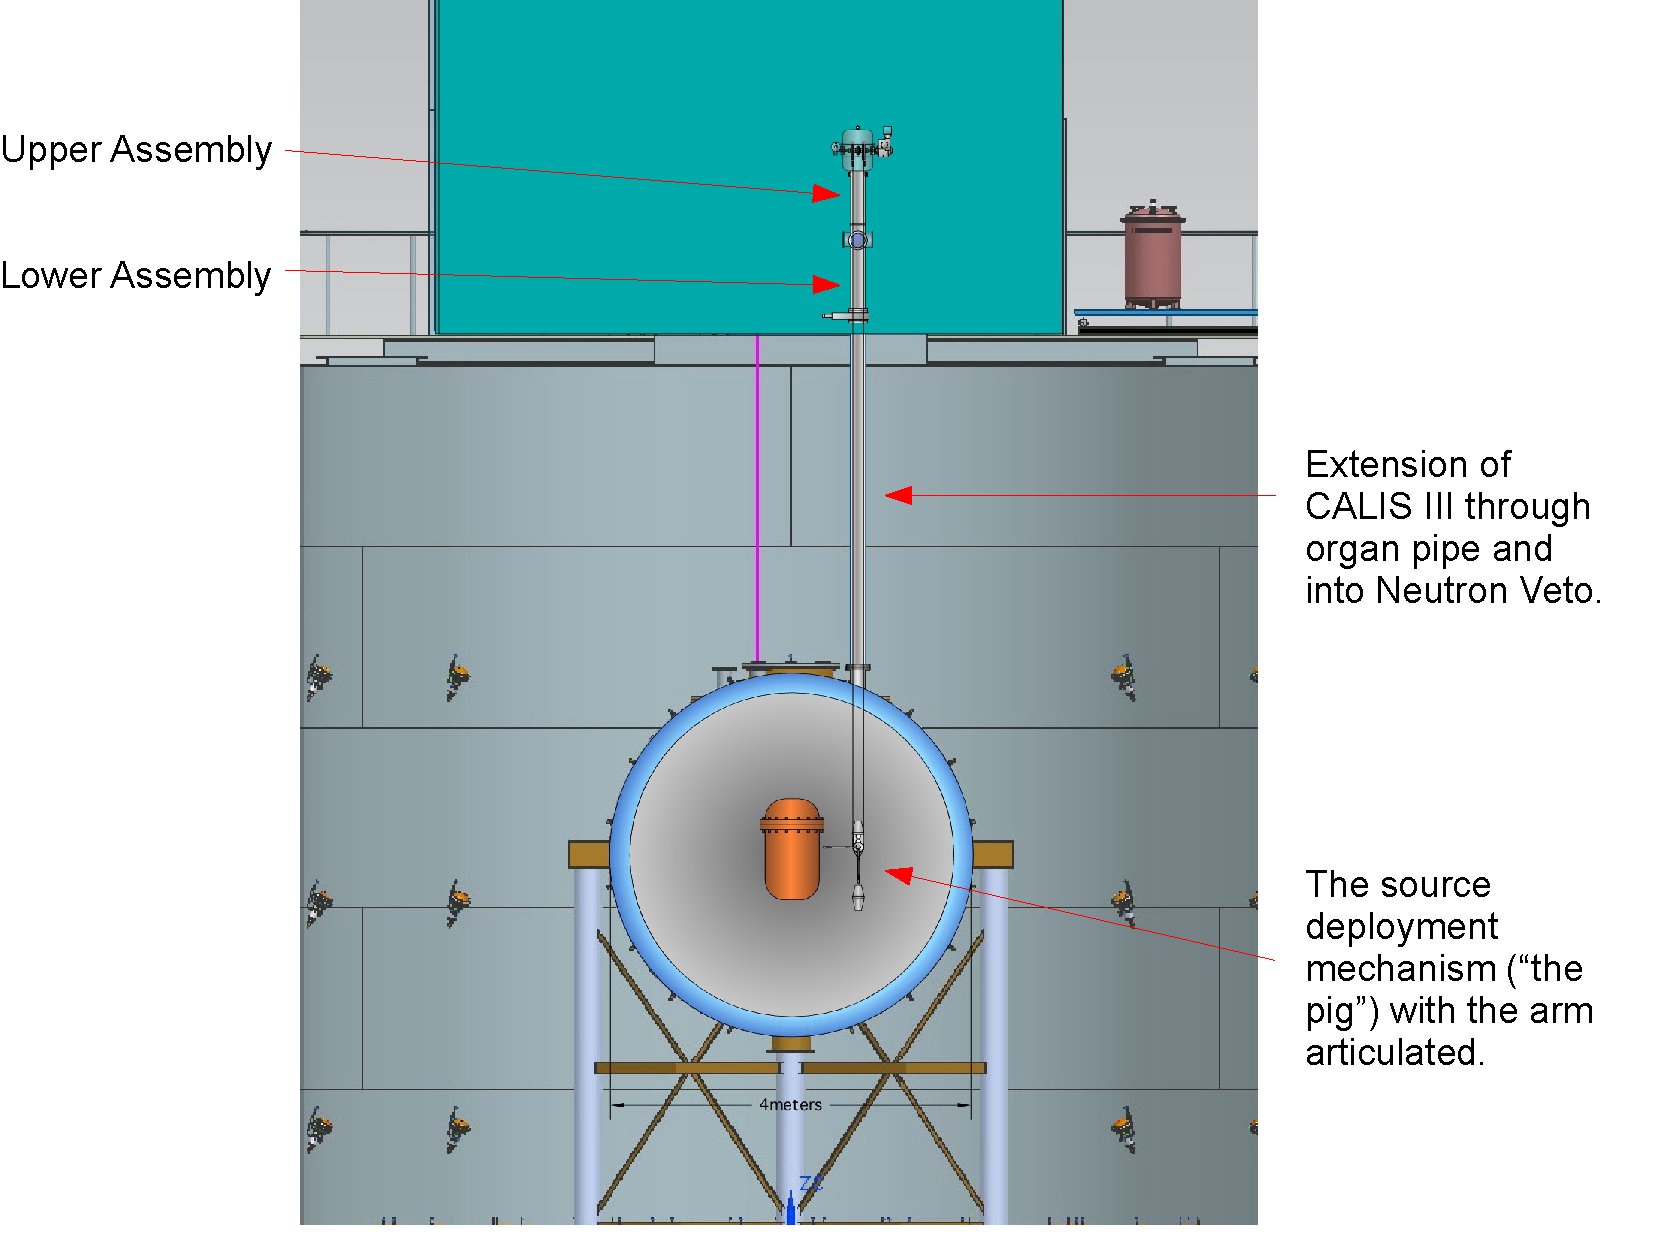
\includegraphics[width=7.5in]{Figs/wholeAssembly_insideDetectors}
 \caption{A conceptual drawing of CALIS III installed in CRH and deployed in LSV next to the cryostat. The CALISIII extends into LSV during calibration only. Z position is controlled via stepper motor located in the upper assembly. Raising of the source arm (shown in both vertical and ariculated, horizontal position) is achieved by manual raising of the cable for a fixed length. Azimuthal rotation of the source is achieved by rotating the upper assembly and the source deployment mechanism with respect to the lower assembly. This can be done during deployments as the system holds pressure during the entire process. CALIS III is parked inside upper and lower assembly when not used for calibration. Gate valve at the top of the organ pipe remains closed except during calibration campaigns.}
\label{fig:wholeAssembly_insideDetectors}
\end{figure}


\begin{figure}[htbp]
 \centering
 \includegraphics[width=5.5in]{Figs/CALISDimensions3}
 \caption{Mechanical drawing of the full device with dimensions in inches (centimeters) shown. The arm length is variable, the 40.31\,cm (15.87\,inch) long arm is shown in the figure.}
 \label{fig:CALISDimensions3}
\end{figure}


\begin{figure}[htbp]
 \centering
  \includegraphics[width= 8.5in]{Figs/sourcePod_arrows}
  \caption{The pig-support for the arm and the source holder.}
  \label{fig:sourcePod_arrows}
\end{figure}

 \subsection{The Lower Assembly} \label{The Lower Assembly}
 \paragraph{}
    The lower assembly is a cylindrical stainless steel enclosure pipe that contains the ports for viewing and accessing the source and the cables on its upper end. The front view/access port can be opened for easy manipulation/handling of the source. Below the view port is a sealed connection that has an o-ring seal and uses a ring clamp to compress the seal. The clamp can be slightly loosened to allow the entire upper assembly with the pig to be rotated with respect to the lower assembly and the detector. Refer to Fig. \ref{fig:Rotation2} for a conceptual description of the device rotation with respect to the detector and the assemblies). The angle rotation is read out from the measuring strip. The ring clamp and the measuring strip are shown in Fig.~\ref{fig:ring_clamp}. During the rotation in the xy-plane, light and air tightness are preserved. Thus, the rotation of the pig can be performed, while the pig is deployed next to the cryostat (and open  gate valve).  The lower assembly is connected to the gate valve on top of the organ pipe in CRH.  The distance from the center of the viewing port to the top of the gate valve flange is 74.85\,cm (29.47\,inches). This distance was based on a person sitting comfortably in a chair while handling the source.  Fig. \ref{fig:lowerAssembly_dimensions} shows the dimensions of the lower assembly and the upper and lower assemblies connected as they will be in CRH in comparison to a person of average height.   When the source arm is centered in the view port, the view port may be opened for handling of the source.  This is considered the home position for the pig.  

\begin{figure}[htbp]
 \centering
  \includegraphics[width=6.0in]{Figs/Rotation2}
   \caption{Shows the top view of the upper assembly and how the azimuthal rotation of the source is achieved by rotating the whole upper assembly with respect to the lower assembly and the entire detector.}
  \label{fig:Rotation2}
 \end{figure}

\begin{figure}[htbp]
 \centering
  \includegraphics[scale=0.5]{Figs/RingClamp.jpg}
  \caption{Ring clamp  with the angle measuring strip shown below. In order to perform azimuthal rotation, ring clamp is slightly loosened, and the entire upper assemby is rotatated with respect to the lower assembly, along with the pig. The angle of rotation is read out from the strip that goes around the pipe. }
  \label{fig:ring_clamp}
\end{figure} 
	

%\begin{figure}[htbp]
% \begin{minipage}[b]{0.5\linewidth}
%  \centering
%  \includegraphics[width=\linewidth]{Figs/Rotation2}
%  \caption{Shows the top view of the upper assembly and how the azimuthal rotation of the source is achieved by rotating the whole upper assembly with respect to the lower assembly and the entire detector.}
%  \label{fig:Rotation2}
% \end{minipage}
% \hspace{0.5cm}
% \begin{minipage}[b]{0.5\linewidth}
%  \centering
%   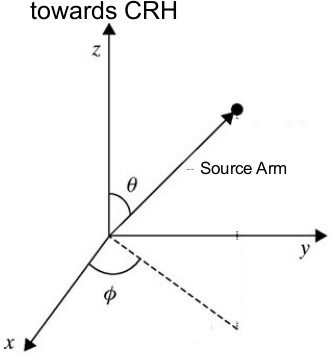
\includegraphics[width=\linewidth]{Figs/coordinate_system}
%  \caption{Coordinate System used.  Shown here for reference.}
%  \label{fig:coordinate_system}
% \end{minipage}
%\end{figure}

\begin{figure}[htbp]
 \centering
  \includegraphics[width=7in]{Figs/lowerAssembly_dimensions}
  \caption{Shows the upper and lower assemblies together as they will be installed in CRH next to a welder for perspective. additional 20\,cm (8\,inch) long pipe section has been added above the viewport to accommodate longer arms inside the upper assembly. }
  \label{fig:lowerAssembly_dimensions}
\end{figure}



	
 \subsection{The Upper Assembly} \label{The Upper Assembly}
 \paragraph{}
  The upper assembly is a stainless steel cylindrical enclosure that houses the drive mechanism and the gear drive for the cables. The raising and lowering of the source is controlled by a servo motor drive which is operated via a LabVIEW interface (Sec. \ref{LabView}).  The motor controls z positioning of the source by simultaneously unwinding and winding a pair of cables  that the pig is attached to.  We are able to specify in LabVIEW a z position that we want the source to be in and command it to go there.  In order to move up or down in z motor is given a certain number of steps to go. There is a translation table that gives correspondence between each z positiona and number of steps on the motor. The motor has an absolute encoder and step position is never lost even in the case when the motor loses power. When the pig has reached its home position within the upper assembly it will stop.  However, if the top of the pig continues past its home position (based on the number of steps given), it will not be able to pass its home position thanks to the upper limit switch that will be triggered in that case. When contact is made with the switch, it will trip the upper limit and open the circuit, turning off the 24 Volts line powering the motor.  This would be considered a system failure and the problem will need to be understood and corrected before continuing.   
 Fig.~\ref{fig:limit_switch} shows the schematic of the connection between the limit switch and the motor.
 
  %See Fig. (working on getting this) for circuit diagram.  
  
     
 %add limit switch diagram here!!!
 %caption for limit switch diagram---
 	%For the arm retraction switch: the pointer must be pointing to 0 (the arm is in its vertical position) to get a permit for the pig to move. This pointer should never enter the red zone.  
 	

\subsection{Deployment Mechanism} 
two cables

 	
 	
  The articulation of the arm is operated manually.  A hand wheel is located outside of the device (shown in Fig. \ref{fig:gearDrawing} on the left side) allows the user to manually raise the arm to its horizontal position. Section \ref{The Pig} details the use of the hand wheel to articulate the arm.  





To prevent the system from being moved while the arm is articulated, an arm retraction switch has been installed. If the arm is not in the vertical position, the switch will be open and there will be no power to the motor (no power in the 24 Volt line), as can be seen in Fig.~\ref{fig:limit_switch}.  Without the 24 Volts, the pig can not be moved up or down.  Fig \ref{fig:gearDrawing} is an image of the upper assembly inner components with the hand wheel on the left side and the servo motor on the right.  Fig.\ref{fig:sideView_upperAssembly_components} provides a side view of the upper assembly inner components.  
 
\begin{figure}[htbp]
 \centering
  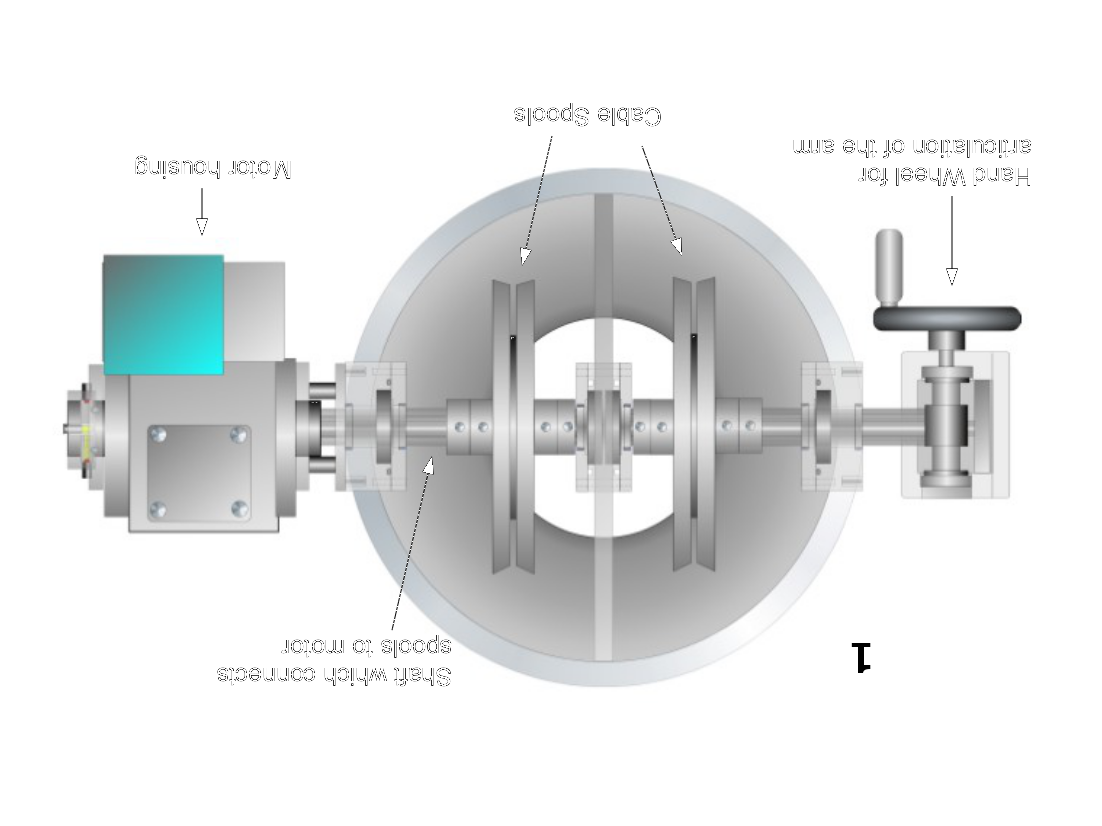
\includegraphics[width=6in]{Figs/gearDrawing}
  \caption{Looking down on the top of CALIS III and inside the upper assembly: the components and drive mechanism are shown. The hand wheel is on the left connected to one of the spools only. The next parts going from lft to right are the two cable spools and then the sealed motor housing. }
  \label{fig:gearDrawing}
\end{figure}

\begin{figure}[htbp]
 \centering
  \includegraphics[width=7in]{Figs/sideView_upperAssembly_components}
  \caption{The photo of the hand wheel and top of the upper assembly. The two cable spools are visible inside.}
  \label{fig:sideView_upperAssembly_components}
\end{figure}
	
 \subsection{LabVIEW Interface} \label{LabView}
 \paragraph{}
 Graphical user  interface (GUI) to the stepper motor is realized with the LabVIEW, graphical programming language.  The program communicates with the drive mechanism and the absolute encoder.  The vertical movement of the pig is controlled via LabView.  The interface gives the z-position of the pig according to the absolute encoder, hereafter called the step position.  Step position 0 is the home position of the pig.  Starting and stopping of the pig is controlled in this interface.  LabVIEW also shows a plot of the motor current vs time as the pig is moving.  In order to command the pig to move, the desired step position is typed in, followed by a  click on the Start Move button. If, at any time in the movement of the pig, you wish to stop the pig before it reaches the set step position, then click the Stop Move button.   The photo of the current GUI is shown in the Fig.~\ref{fig:GUI}. 

\begin{figure}[htbp]
 \centering
  \includegraphics[width=7in]{Figs/GUI.jpg}
  \caption{The photo of the GUI used to control the motor.}
  \label{fig:GUI}
\end{figure}	
	
 \subsection{The Pig} \label{The Pig}
 \paragraph{}
The pig (Fig. \ref{fig:sourcePod_arrows}) contains the support structure for the arm which holds the source at its end.  This piece is equipped with tapered cones on the top and bottom that ensure that the ends do not get snagged on inner edges of the organ pipe as it is moving up and down. It is attached to the assembly by the two cables.  Swivel hooks are employed in the attachment of the cables to the pig that allow the cables to move freely and not get tangled.  There is a chain that goes from the swivel hook around the gear to the second swivel hook. In the center of the gear is a custom designed and fabricated source arm pivot that the arm is attached to and that rotates together with the articulation gear visible in the center of the pig. See Fig. \ref{fig:SourcePod2} for an image of the arm raised to its horizontal position.  
 
\begin{figure}[htbp]
 \centering
  \includegraphics[width=3.2in]{Figs/SourcePod2}
  \caption{The photo of the pig with the arm in its horizontal position.}
  \label{fig:SourcePod2}
\end{figure}

\subsection{Source arms}
  For articulation, there is currently a choice of three arm lengths---40.31\,cm,  57.15\,cm and 62\,cm.  Each of these lengths are measured from the center line of the organ pipe to the end of the source holder.  The arm lengths, 57.15\,cm and 62\,cm are intentionally made too long as they will be used to determine the exact location of the cryostat; some uncertainty in the cryostat's z and lateral position exist at the level of 3 - 4\,cm. The organ pipe we intend to use is 81\,cm distant from the cryostat center (and the geometric center of the LSV sphere) as measured from the center line of the organ pipe. The cryostat is 32\,cm in radius, which leaves a distance of $\sim$49\,cm to be reached  by the arm.  The articulation of the arm is operated via a hand wheel located on the side of the upper assembly close to the top.  By rotating the hand wheel, one of the cable spools inside the upper assembly will rotate which pulls up on one of the cables attached to the pig and shortens it for the length equal to the one quarter of the gear curcamference (which is 10\,cm).  As a result, the chain at the bottom of the cables engages the articulation gear (see Fig. \ref{fig:sourcePod_arrows} for an image of the articulation gear) on the pig and raises the arm to horizontal.  The chain has a guard rail that ensures that chain can never come of the gear. Thus, in the process of articulation the entire pig along with the source arm shifts up for 10\,cm.  See Fig. \ref{fig:pigAndCables_fullView} and  Fig. \ref{fig:sourceArmRotation} for a closer look at how CALIS III articulates the arm. In order to determine the degree of articulation of the arm, a protractor is placed next to the hand wheel.  This protractor and the hand wheel are calibrated together for an accurate reading of the articulation. The reading of the protractor dial is different at different heights and calibration table obtained from the tests is used to determine the dial setting necessary to articulate the arm to horizontal position. We have adopted a spherical coordinate system for the rotation of the system and the articulation.  Articulation of the arm is measured in $\theta$ from the z-axis; when the arm is fully articulated, it is at 90$^{\circ}$ and when it is in its vertical position it is at 180$^{\circ}$.  As mentioned in Sec. \ref{The Lower Assembly}, the rotation of CALIS III is done in the xy-plane which corresponds to the azimuthal direction, a rotation in $\phi$.  See Fig. \ref{fig:coordinate_system} for details. 
  
\begin{figure}[htbp]
 \centering
  \includegraphics[width=7in]{Figs/pigAndCables_fullView.png}
  \caption{CALIS III showing the inner workings of the articulation of the arm and the arm in its vertical position. }
  \label{fig:pigAndCables_fullView}
\end{figure}

\begin{figure}[htbp]
 \centering
  \includegraphics[width=7in]{Figs/sourceArmRotation.png}
  \caption{Technical drawing showing the mechanism behind the rotation of the arm. }
  \label{fig:sourceArmRotation}
\end{figure} 


\subsection{Degrees of freedom of the system}
\begin{figure}[htbp]
 \centering
  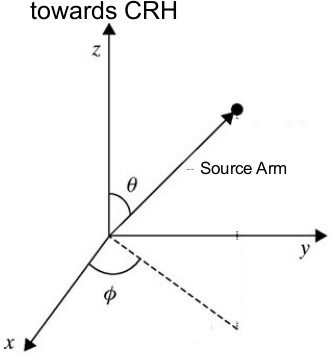
\includegraphics[scale=0.9]{Figs/coordinate_system}
  \caption{Spherical coordinate system used for establishing the direction of the rotation of CALIS-III and the articulation of the source arm. $\theta$ is kept at 90$^{\circ}$ when arm is articulated, and at 180$^{\circ}$ when dearticulated. $x$-axis is the direction toward the center of the detector. }
  \label{fig:coordinate_system}
\end{figure} 
	
 \subsection{Safety features} \label{Safety Features}
  \paragraph{} 
 CALIS III offers various safety features to ensure that the device runs smoothly, no components (especially sources) are lost inside the detector, avoid any contamination of the detector by dirty or incompatible materials, maintain pressure and avoid introduction of oxygen or water in contact with the LS and TMB, operation in the volume that excludes possibility of contact with PMTs or light pulsers (pacman) attached to each PMT.
 
 \begin{itemize}
  \item{Drive Mechanism}
 
   The drive mechanism is a stepper motor that has an integrated absolute encoder providing the location of the source at all times, even in the event of a power failure. The torque of the servo motor is limited in case of an unexpected load.

 \item{Magnectic Break}
 
  In the event of a power failure, the magnetic break ensures there is no movement of the pig. 
  
  \item{Speed Reducer}
  
  The speed reducer (gears) is a double worm gear design. The primary worm gear has a 50:1 reduction and the secondary worm has a 82:1 reduction. The input speed of the servo motor is 2400 RPMs and the output is 0.6 RPM and has the weight capacity of 148 lbs. In the event of a power failure the speed reducer has the ability to hold the load at any position without back drive. The speed of the motor has been limited to 0.4\,cm/s which minimizes any lateral oscillation of the pig during lowering and raising the source. Additionally, this is the maximum speed at which the motor is not overheating.
	
\item{Manual retraction system}

In case of complete motor failure while the source is deployed, it is possible to manually retract the pig back to its home position and close the gate valve. The motor is disengaged, and wrench is used to manually wind the cable back onthe spools and retract the pig back above the gate valve.

\item{Cable strength and cable termination}

The cables holding the pig have been rated for loads over 590\,kg, while the weight of the pig is at the level of 10-15\,kg so well below the breaking strength of the cable. The cable terminations have been crimped with stainless steel crimps and swivel hooks conneted to the thimble of the cable termination.

\item{Cable length}
The cable length has been established so that the maximum depth at which the pig can be deployed is above the level of the PMTs. In case, the command is given to deploy to greater depth, the cable completely unwinds and then rewinds in the opposite direction, which then effectively retracts the pig to a higher z-position until the preset motor count of steps is reached. 

%% is this true?

\item{verticality of the organ pipes}
electrical contact was made, but still quite straight. Dimensions of the organ pipes? Also interesting to report above...


   
\item{Upper limit switch}

There is a limit switch inside the upper assembly that will cut the power to the motor if the pig starts to move above its designated home position.

\item{Articulation retraction limit switch}

Arm retraction limit switch cuts the power to the motor as soon as the arm is not vertical. In this way, any possibility of retracting the arm into the organ pipe while articulated has been eliminated.

\item{Choice of materials}

All materials that come into contact with LS and TMB or their vapors, have been made out of stainless steel, teflon and viton that have been certified as safe in contact with the LS and TMB.


\item{Light covers on the view ports}

All viewports have  very tightly fitting covers. Additionally, the main viewport cover will additionally be held in place with clamps to avoid any possibility of accidently exposing the LSV to excessive amount of light. 
     
\item{Leak tightness of the source holder}

 The source is placed inside a stainless steel container that has an o-ring seal (made out of viton) during calibration. The container has been tested at Fermilab to be helium leak tight.  

\item{tapered cones}
Tapered cones at the top and bottom end of the big minimize the risk of the pig getting tangled while moving up or down. This is a safety precaution, since the organ pipes are free of cables or sensors and 





\item{Securing of the source}

All connection points for the source and arm have been secured with two push locking pins that cannot be disengaged without person pressing the pin. 
The source holder is held in place via a locking mechanism and two locking pins (see Fig \ref{fig:sourceHolder_locking} and Fig. \ref{fig:sourceAttachmentParts}).  When the source is attached to the arm, the source container must be slid over a protruding pin. There is a sliding locking mechanism that interlocks onto the pin. Once the source is locked into position there are 2 additional locking pins that are put into place (one above and one below the source holder pin), each of which have a button that must be depressed in order for the pins to be released.  See DocDB \#858 for two movies in which this mechanism is demonstrated. In addition, the source holder and the 2 locking pins will all be tethered from outside the view port until they are locked in place eliminating the possibility of accidental falling.  The tethering will happen before installation of the source and before the removal of the source. The cables used to tether the pins and the source holder during installation and removal will be detached after installation and prior to deployment to avoid the possibility of the arm getting entangled.  
 
\begin{figure}[htbp]
 \centering
 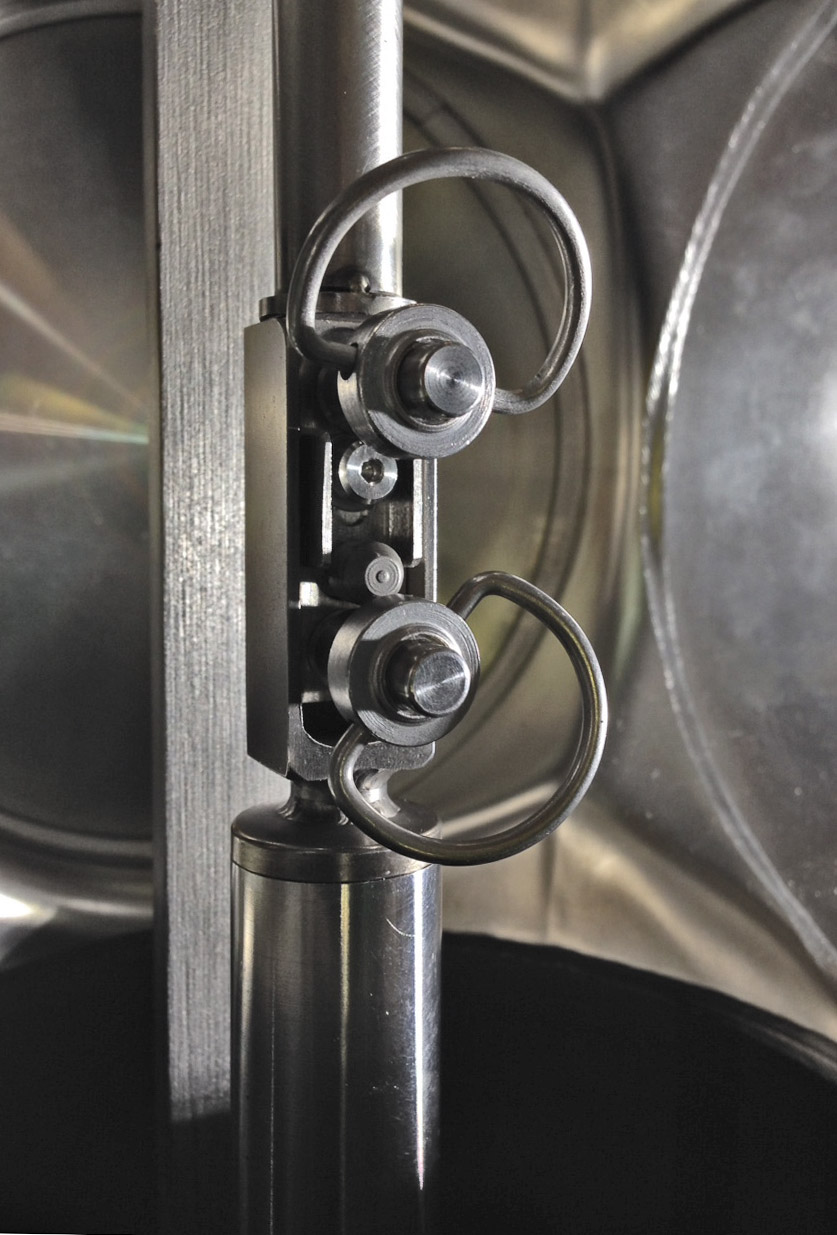
\includegraphics[width=3.2in]{Figs/sourceHolder_locking}
 \caption{Locking mechanism for the source holder. This photo shows two push pins that ensure that the sliding pin stays in place and the the source holder cannot under any circumstances get detached from the arm.  The only way to remove the push pins is to depress buttons on each of them by hand. }
 \label{fig:sourceHolder_locking}
\end{figure}

\begin{figure}[htbp]
 \centering
  \includegraphics[width=7in]{Figs/sourceAttachmentParts}
  \caption{Components of the source attachment mechanism. Central image shows how the pin that holds the source holder slides down and prevents the source from getting loose.  The slide pin is locked in place by two push pins shown in Fig. \ref{fig:sourceHolder_locking}}
  \label{fig:sourceAttachmentParts}
\end{figure}

\end{itemize}

 \subsubsection{Light Tightness}
 
   In order for CALIS III to be light tight, all view ports have light tight covers for when the organ pipe gate valve is open. When any view port or access port is opened, the gate valve must be closed, eliminating the possibility of leaking light into the veto. Additionally, all seals of CALIS III will be tested for leaks and confirmed to be helium leak tight. The gas tightness will be validated again after installation on the gate valve with gate valve closed. 
	
 \subsubsection{Vacuum evacuation and nitrogen purging}
 \paragraph{}
   One of the most important features of this system is making sure that the TMB and PC residue on the device are extracted from CALIS III prior to opening access ports to exchnage source or arms. This is  important for  safe working level of the people involved and for the detector.  This can be addressed through a system evacuation and nitrogen purge.  To accelerate the removal of the TMB in the scintillator fluid residue that is left after a deployment, CALIS III will undergo an evacuation with a vacuum pump. By lowering the pressure inside of CALIS below the vapor pressure of the TMB, it will cause the TMB to outgas and be removed through the vent line of the vacuum pump. An additional step to remove the TMB is to purge using N$_{2}$.  We will need to limit the potential flow rate of the nitrogen to ensure that an ODH (Oxygen Deficiency Hazard) condition is avoided in CRH.  Only once this is accomplished, will the view port be allowed to be opened and the source handled.     
  
The entire CALIS III  has been tested at FNAL  to hold pressure.  The system will be tested again after installation on the gate valve.

\section{Installation location of CALIS in CRH}
The CALIS will be brought inside CRH semi-assembled and then the full assembly of CALIS will take place inside the CRH. There the system will be hung on the crane in order to perform a reduced set of validation tests to verify te CALIS performance after the clean assembly and in its final configuration for calibration.    Once these tests show satisfactory performance, the device will be installed in the organ pipe port, visible in Fig. \ref{fig:CRHLocation}.  

\begin{figure}[htbp]
 \centering
 \includegraphics[width=7in]{Figs/CRHLocation}
 \caption{The red arrow indicates the proposed location for installation of CALIS III within CRH. This is organ pipe N11C.}
 \label{fig:CRHLocation}
\end{figure}
 
\section{Testing} \label{Testing}
 \paragraph{}
  
 Testing of CALIS has been performed at FNAL in the second half of August and first half of September 2014. CALIS was installed in a building with the high bay, on a high platform, so that the full length deployment tests could be performed. The tests are repeated at LNGS prior to cleaning the system, and some validation tests are foreseen at the time of installation in CRH.  Several different tests have been conducted:
\begin{itemize}
 \item{Motor controls debugging}

    LabView interface with the motor controls has been verified and responds to all commands (starting/stopping of vertical deployment) as expected.  Motor current can be read from the GUI and shows opposite signs if motor is rotating in one vs the other direction as an additional sign of the  motion direction.

\item{\bf Vertical (z) position accuracy and repeatability}
{\bf Procedure:} As a first step in testing the reproducibility of the z position as a function of step position,
a baseline relationship between step number and vertical displacement was determined. First, the distance
from the floor to the bottom of the pig was measured using a laser ranger, starting from what was found
to be the lowest pig position (fully deployed). The bottom of the pig was covered with tape to serve as a
target for the laser ranger. After this first measurement, the pig was raised, stopping approximately once
every minute to record the step position and measure the corresponding z distance, until it reached the home position (fully retracted). Subsequently, in the following test runs, the pig was again sent to each of these steps, the z position was measured with the laser ranger, and all values recorded. After 2 runs in which every step which had been recorded in the baseline was measured, it was realized that recording so many data points would require several weeks to complete the testing. The number of data points was then cut in half for 4 runs, and cut in half again for the remaining 24 runs for a total of 31 runs.

{\bf Results:} The vertical displacement of the pig was found to be extremely consistent, with no apparent
drift due to slippage or any other effect. The average uncertainty of each z coordinate was found to range
between 1-2\,mm, numbers consistent with the uncertainty of the laser ranger and the unevenness of the tape on the bottom of the pig. Fig.~\ref{fig:z_test} shows the correspondence between the z position and stepper motor count exibiting a smooth function with no visible variation of the points from the fit. No measurable slippage of the cables or accumulated offset of the stepper motor count and z position was observed during the repeated tests.

\begin{figure}[htbp]
 \centering
 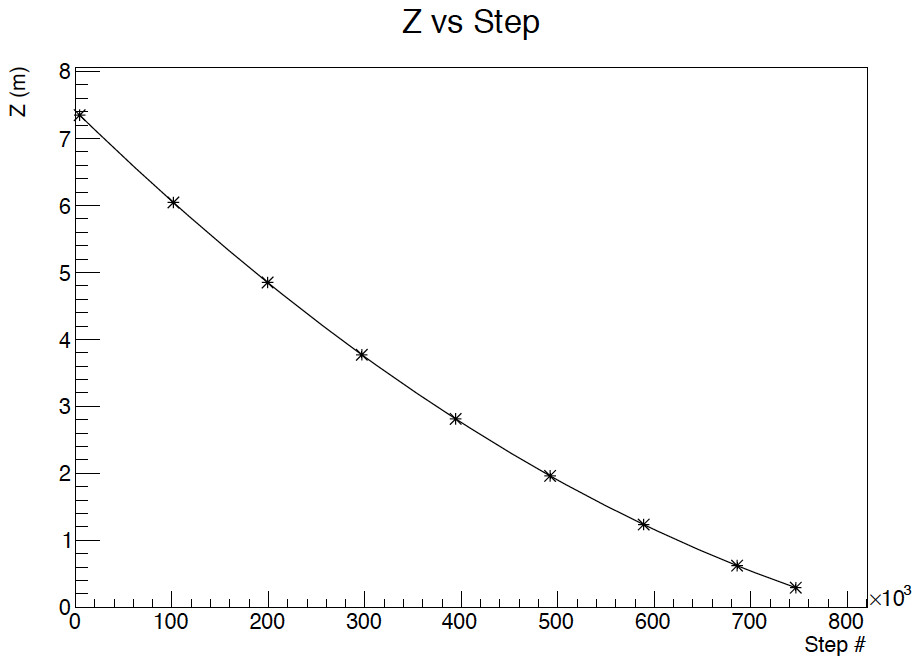
\includegraphics[width=3.2in]{Figs/Z_positioning_test}
 \caption{Plot of the z position of the pig vs the step position of the motor.}
 \label{fig:z_test}
\end{figure}


\item{\bf Lateral motion during depoyment}

The pig is deployed at a very low speed, barely visible to the naked eye. It takes about 30 minutes to deploy the system from its home position to the level of the TPC, approximetely 7\,m below. As a result, there is a negligible level of lateral motion during vertical motion at the level of 2-3\,mm. The motor has a very slow acceleration (both positive and negative) that eliminates any visible jitter at the beginning or at the end of the motion.

\item{\bf Articulation tests}

{\bf Procedure:} Arm is articulated using a manually operated hand wheel.  The arm is articulated to 90$^{\circ}$ every time. This corresponds to a different reading of the dial connected to the hand wheel for different z-position. The second calibration table required, gives correspondence between the z height and required reading on the dial to articulate to 90$^{\circ}$. 

In order to verify the consistency of articulating to the same rotation angle of 90$^{\circ}$ at all needed positions,  full articulation of the arm at different z positions was tested. For this test at Fermi lab, two vertical positions were chosen: one approximately at the center of the cryostat mock-up, and one at the lowest known position of the pig. At each position, the arm was articulated and
the required angle recorded. In order to ensure that the arm was fully articulated, a level was placed on the
arm and required to be horizontal. Additionally, the vertical displacement of the pig was measured before articulating the arm, while the arm was articulated and after the arm was again vertical. Between runs, the
pig was sent all the way back to the home position to simulate the actual deployment conditions as closely as possible. The process was repeated 10 times  (10 runs) to check consistency of articulation among independent runs.

{\bf Results:} During driving the pig up and down through the whole length of the cable, it was noticed that the arm did not return to a perfectly vertical position, which was especially noticeable when the pig was in the home position. To document this, photos were taken each time the arm was de-articulated and when it was in the home position. The hand wheel was renormalized to zero several times, but this offset continued to reappear. It did not seem to progress, however, and remained at approximately the same angle, as can be seen from the photographs in Fig.~\ref{fig:art_offset1}, Fig.~\ref{fig:art_offset2}, Fig.~\ref{fig:art_offset3} and Fig.~\ref{fig:art_offset4}. In all tested cases, offset was relatively small and did not create a problem for retracting the pig inside the lower assembly pipe and to the home posiiton. 

 It was noted that some of this offset was due to the fact that the pig is allowed to swing freely. When articulating the arm, one cable on one side of the pig is raised. This causes the pig to also slightly move in the direction of the articulation. After the
arm is dearticulated, the arm returned to vertical according to the hand wheel, but not according to visual
inspection and use of a level. Part of the offset is because the pig moved in the direction of articulation and
during dearticulation it did not return to its original position. It seemd to get stuck at a slight offset, but a
small tap on the side of the pig returned it to its original position. Additionally, the full arm articulation did
not occur at exactly the same angle each time. This was most noticeable in the lowest pig position, which
had an uncertainty of $\pm$2$^{\circ}$ (as measured on the hand crank). While searching for the cause of
this, it was discovered that a portion of the cable had been stretched during earlier load testing (cable was put under 300\,kg load to test the strengh of the crimp connections), which may have
led to a slightly uneven extension / retraction of the cables, as well as tension at certain points along the
line. The cable was unwound from the spool and allowed to return to its original length.
 The source arm had less of an offset in the vertical position than it had before adjusting the cable, although it was not perfectly straight. The articulation angle as read on the hand crank remained approximately the
same. This test will be completely repeated at LNGS with the final length of the cable in question.

\begin{figure}[htbp]
 \centering
 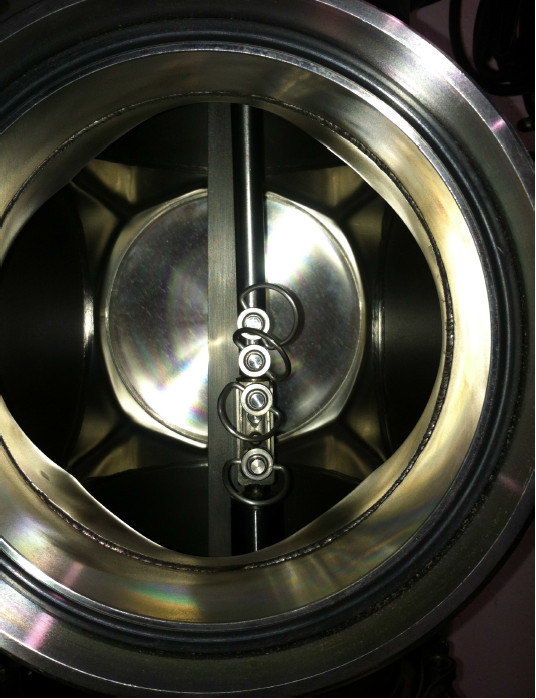
\includegraphics[width=3.2in]{Figs/ArticulationOffset1.jpg}
 \caption{Image of the pig in the home position. The offset of the arm is clearly visible, but below the level that creates problem for motion inside the organ pipe.}
 \label{fig:art_offset1}
\end{figure}

\begin{figure}[htbp]
 \centering
 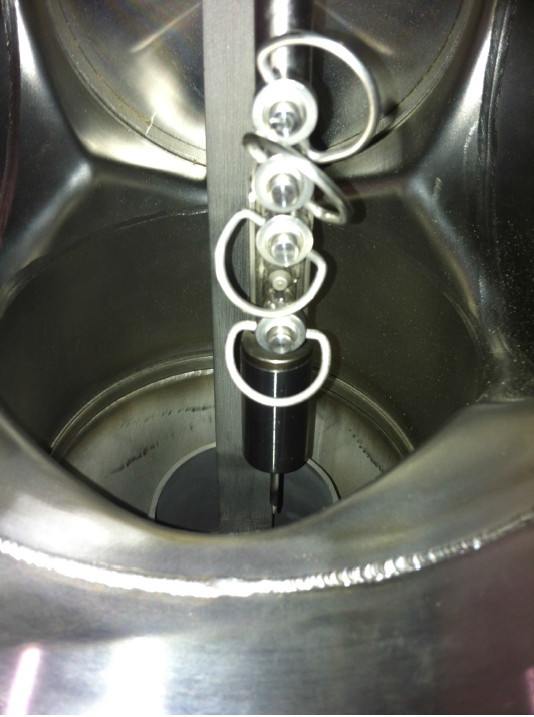
\includegraphics[width=5in]{Figs/ArticulationOffset2.jpg}
 \caption{Another image of the pig in the home position, this time looking down into the lower assembly. Again, note the offset of the arm.}
 \label{fig:art_offset2}
\end{figure}

\begin{figure}[htbp]
 \centering
 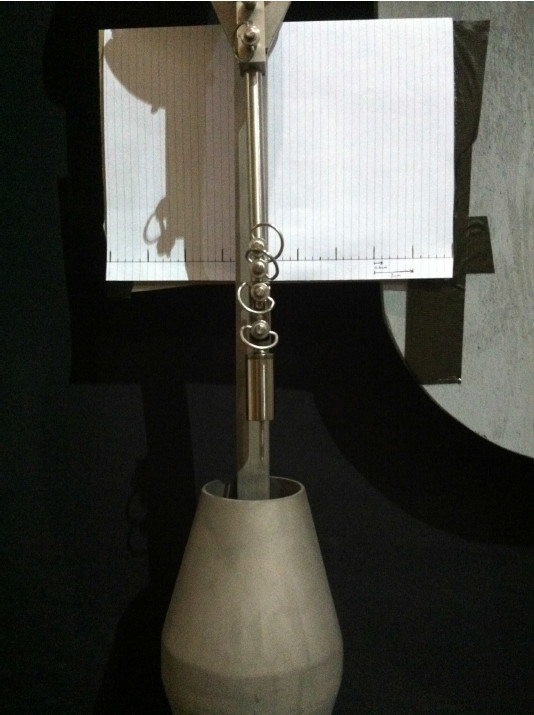
\includegraphics[width=5in]{Figs/ArticulationOffset3.jpg}
 \caption{Image of the pig next to the cryostat mock-up and the ruler used in the horizontal swing test. Note the offset of the arm.}
 \label{fig:art_offset3}
\end{figure}

\begin{figure}[htbp]
 \centering
 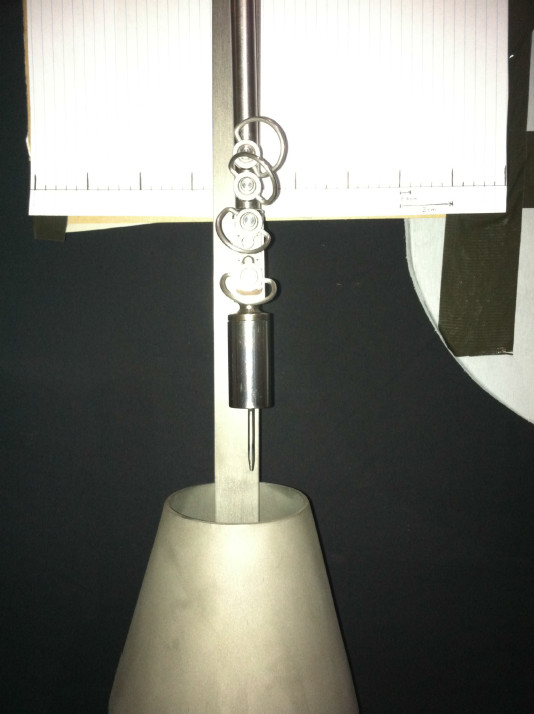
\includegraphics[width=5in]{Figs/ArticulationOffset4.jpg}
 \caption{Again, the pig next to the cryostat mock-up and ruler, a close-up of the arm offset.}
 \label{fig:art_offset4}
\end{figure}

\item{\bf Magnitude of horizontal swing during articulation}

{\bf Procedure:} To measure the horizontal swing of the system during articulation, a 'ruler' was devised and
attached to a mock-up of the cryostat, with a smallest unit of measure of 0.6 cm. The pig was then sent to
the step position where the ruler could be utilized. While the arm was articulated and de-articulated, video
was taken of the swing of the pig.

{\bf Results:}  Anaylsis of the video shows that the pig swings approximately 1.5\,cm during articulation. The articulation is very slow and the swing is very slow. It takes a couple of minutes for the arm to come to complete rest.
    
 \item{Electrical contact test for purpose of determining position of cryostat within the neutron veto}
  
\item{\bf Procedure:} One of the main goals of the first deployment of CALIS-III is to determine the location of the cryostat within the neutron veto as there is a 3-5\,cm positioning uncertainty from construction in the xy-plane and 2\,cm in the z direction.

One test to confirm the position of the cryostat is to electrically connect an arm of the pig to the cryostat. At Fermilab, the electrical contact test was simulated to prove the validity of the idea. The pig was fitted
with a special arm comprised of a stainless steel tube, and the cryostat mock-up received a stainless steel
block attached to it via screws. At the top of CALIS-III, a wire was connected between the lower assembly
and the output of a voltmeter. A wire from the stainless steel block was connected to the voltmeter input. The special arm was first articulated and then the whole assembly was rotated in the azimuthal direction in
order for the arm to make contact with the stainless steel block as can be seen in the Fig.~\ref{fig:electricalContact}.

{\bf Results:} When the arm made contact with the square, the completed circuit was indicated by the
voltmeter. Contact of the arm with the steel block was also verifed by visual inspection. The rotation and
contact was repeated several times and at each contact, the voltmeter registered (by beeping) the connection.

\begin{figure}[htbp]
 \centering
 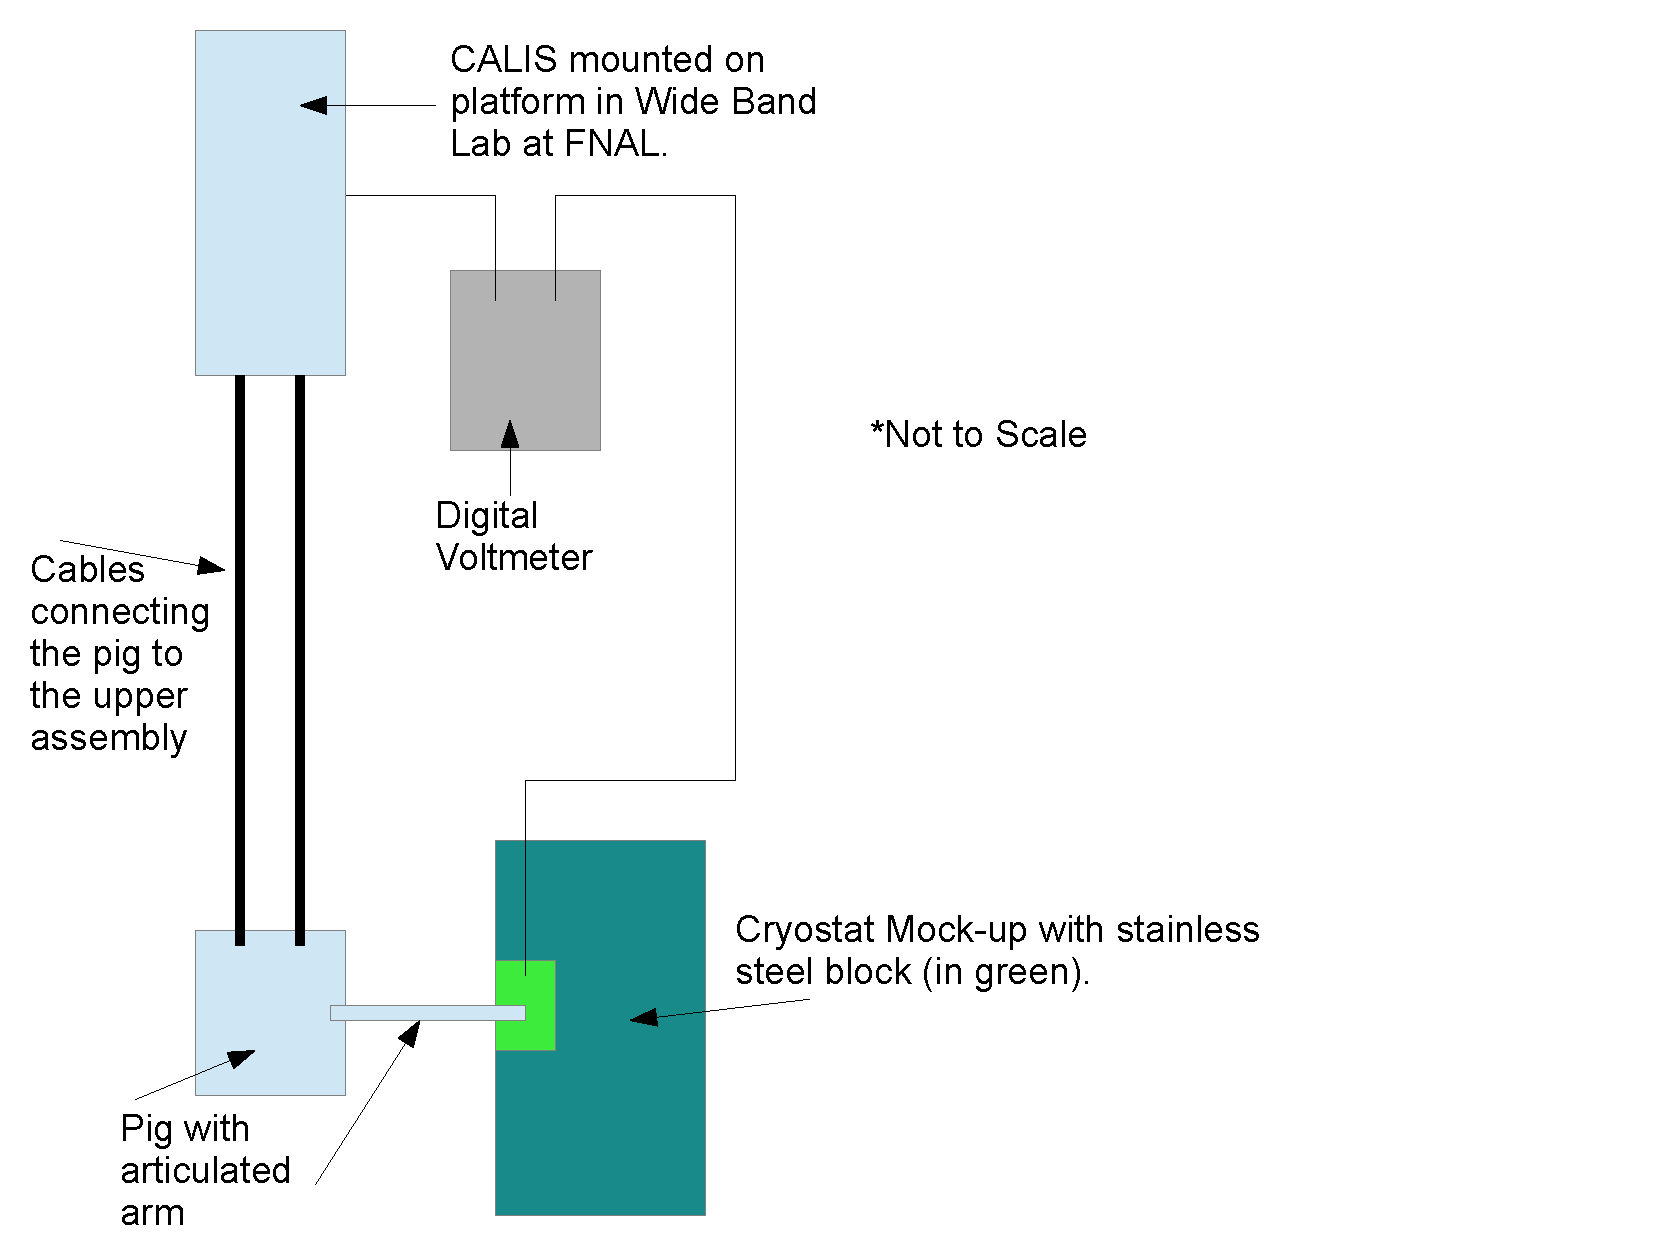
\includegraphics[width=7in]{Figs/electricalContact_FNALtest_diagram}
 \caption{Diagram of the electrical contact test performed at FNAL.}
 \label{fig:electricalContact}
\end{figure}

\item{\bf Functionality of the safety features}

Both the upper limit switch and the arm retraction switch have been tested and operated as expected. 
\begin{itemize}
\item
The pig did not move above the home position, despite the command to move up in z as the power was cut to the motor. 
\item
No z-movement was possible prior to retraction of the arm to the vertical position by the hand wheel. We verify that the arm is vertical by verifying that the dial on the protractor next to the hand wheel is pointing at zero mark. 
\end{itemize}
   
 \item{Test Ease and Accuracy of Azimuthal Rotation}
  
{\bf Procedure:} The upper and lower assemblies of CALIS-III can be rotated in the azimuthal direction.  This rotation allows the source arm to move in the xy plane for the purpose of locating the position of the cryostat within the neutron veto.  The rotation needs to be fairly easy to perform and we need to know what kind of precision and accuracy we will have. The rotation of the upper assembly requires one to loosen the clamp between the upper 
and
lower assembly. Once this is done, the upper assembly is manually moved/twisted on its axis in the direction
desired. To test this at Fermilab, the pig was deployed to the level of the cryostat mock-up and the arm articulated.
Then the clamp was loosened and the upper assembly rotated.

{\bf Results:} Despite its substantial weight, the upper assembly was able to be moved on its axis smoothly,
with no jerking or sticking. At the conclusion of testing, a band was axed to the lower assembly and
a pointer to the band was attached to the upper assembly. This is to measure the actual rotation of the
assembly. Due to time constraints, the rotation with the band attached was not able to be done. Therefore
further testing will need to be done at LNGS to determine the accuracy and precision of the azimuthal
rotation.  
 
\item{Helium Leak Tight Testing}
   
The device was tested to be helium leak tight at Fermilab.  
 
\end{itemize}

 \paragraph{}
  A full summary, along with plots, of the testing performed at Fermilab can be found in DocDB \#858.  

After the above described tests at FNAL were finished, it was concluded that \textit{\bf CALIS is in a good operating state} and is ready to be shipped to LNGS for commissioning and calibration.


\section{Commisioning and testing at LNGS}

 The system was shipped sub-assembled to LNGS and arrived in mid-September. Once it arrived, CALIS III was inspected and reasembled. Two rounds of tests are part of the commissioning of CALIS at LNGS: dry tests prior to cleaning and a subset of tests after cleaning the system and prior to installation on the gate valve of CRH. While the goal of the Fermi lab tests was to establish that CALIS is operating as expeced and that all designed safety features are operational, a  goal of the LNGS tests is the final characterization of CALIS to establish the absolute positioning precison of the source. 

The testing location chosen at LNGS allowed full deployment length tests and direct access to both the top of the system where the controls are and to the pig. The chosen locaiton was a tall stairway on the left side of the OPERA detector that has a platform on the fourth floor where CALIS was mounted. A movable platform accessible from the lab floor level was used to raise up to the level of the pig for all planned measurements.   The same set of tests as described above, and a few additional once related to the absolute positioning uncertainty,  have been underway.

 Final characterization of the source positioning must be done with the new cables that have been put on CALIS. The length of the cables was chosen to allow maximum safe, deployment depth that makes any contact with PMTs impossible (according to the engineering drawings of the DarkSide detectors).   Once all dry runs are performed to satisfaction, we will disassemble and clean all components in CR1 as per the normal detector cleaning procedure. After cleaning, the device will be partially assembled and moved into CRH. A subset of validation tests will be conducted from the crane in the CRH and then CALIS will be installed on the top of one of the ate valves.

\subsection{Dry Tests to Perform at LNGS Prior to Cleaning}
All the tests performed at Fermilab are  repeated at LNGS, but the number of runs is reduced as we do not expect to see change in the performance of the motor or the cables. While the tests at Fermi lab confirmed good operational performance of the system, the tests conducted at LNGS are calibration tests whose goal is to make the most precise prediction of the source position during deployment and establish expected uncertainty of that position.  Below is the full list of tests underway at LNGS.

 \begin{itemize}
  \item{Characterization of CALIS-III Positioning} 
 
   The CALIS-III positioning has been characterized with the final cables length. There are two components of the positioning: 

\begin{itemize}
\item
This includes the pig z position as a function of step position.
\item 
The arm 90 degree articulation point as a function of vertical pig position.  
\end{itemize}
This is necessary because, as the cable winds around the spool, the winding radius changes, increasing as the pig is lifted and decreasing as it is lowered.  This means that there is not a linear correspondence between the number of steps and the length of cable deployed.  Additionally, this non-linear dependency causes the amount of rotation required by the hand wheel for full articulation of the source arm to change as a function of the length of cable deployed.     
 
  \paragraph{}
  Every 10,000 steps (order of 10\,cm), we stop the pig and record the z position with the laser ranger, as done during the position reproducibility test at Fermilab.  The arm will then be rotated to 90$^{\circ}$ and the hand wheel position noted for the relevant z locations. The step position for key source locations commonly used during calibration will be determined, including the TPC center, 15 cm above and below the TPC center, and the cryostat top and bottom.  Once these positions have been verified by inputting the step location and measuring the z position and corresponding hand wheel rotation, the results will be formatted for easy use by CALIS-III operators.   
  
\item 
Measure the exact distance of the forward motion (in the direction of articulation) at relevant z positions, as it determins the final distance of the source to the TPC.

\item
Measure if there is any lateral change (in the azimuthal plane) when the arm is articulated at relevant z positions. While none has been observed in the previous tests, it is important to verify this in repeated deployments and articulations.

\item 
Validate the distance that the pig moves up during articulation (measured to be 10\,cm in tests at Fermilab) and verify that this number does not change between repeated articulations.

  \item
Test the arm retraction switch to confirm that the pig cannot be retracted to its home position if the arm is articulated.
  
  \item
During articulation measure the level of the horizontal swing. Confirm it to agree with Fermilab testing.
 
  \item{Determine the time it takes for the arm to reach a stable (non-moving) condition after articulation.}
 
  \item{Test the absolute encoder before and after power failure.}
  \item{Test nitrogen and vacuum systems. Measure the amount of time to evacuate the device and purge with nitrogen.}
  \item{Leak check of upper and lower assemblies.}
  \item{Reproducibility of position in x, y, and z following the full procedure.}
 \end{itemize}
 
\subsection{Tests to be Performed at LNGS after Cleaning}
 After cleaning of the system, we will attach CALIS-III to a crane either in CR1 or CRH to perform a reduced set of tests.  The goal is to confirm that results from tests prior to cleaning and from after cleaning match. 
  
 
  
\section{Proposed Commissioning Plan} \label{Proposed Commissioning Plan}
 \paragraph{}
  Detailed, step by step commissioning procedure is outlined in DocDB\#1021-v1. 
%Once CALIS is installed in CRH, we will need to test gas tightness, light tightness, and evacuation with the vacuum pump.  We will want to move the motors a little bit without opening the gate valve to ensure that all is moving satisfactorily.  Rotation of the whole assembly should be tried at this point and then an alignment will be performed.  We want CALIS to be aligned so that when the arm is articulated it is pointed towards the center of the TPC.  Next, we will open the gate valve and make sure that we can maintain the pressure as it was prior to opening the gate valve.  After that, we will proceed with a 'dummy' deployment (no source in the source holder) down through the organ pipe.  We will start with a low speed and monitor the pressure changes stopping every 5-10 cm to assess the situation.  If all systems are well, then we can increase our descent speed.  At the point of entry into the neutron veto, then we will retract the pig to home position. Once the pig reaches home position, we will again deploy into the neutron veto and attempt articulation of the arm.  We will do the first articulation when we are in optimal viewing from the cameras.  The cameras will be an extra check to ensure that we are at the position that we think we are and be sure we are not going to hit anything.  Once verified, we will dearticulate and continue the deployment, then articulate again when we are near the cryostat and desired testing position.  We will dearticulate and go back to the home position once we are satisfied that the articulation and dearticulation is complete.  As we are lowering CALIS, the DAQ will be monitored to see if there are any electronic noise problems.  We will also monitor to the PMT scalar rates.  By monitoring both the DAQ and the PMT scalars we will be able to tell if there are any light leaks.  
Once all preliminary deployments are completed, we will continue with the cryostat positioning and calibration campaign as outlined in DocDB \#977 for the neutron campaign, DocDB \#978 for the gamma campaign, and DocDB \#960 -- a spreadsheet dedicated to the full campaign.  
  

\end{document}

%\begin{figure}[htbp]
 %\begin{minipage}[b]{0.5\linewidth}
  %\centering
  %\includegraphics[width=\linewidth]{SourcePod}
  %\caption{Source pod--support for the arm and the source holder.}
  %\label{fig:SourcePod}
 %\end{minipage}
 %\hspace{0.5cm}
 %\begin{minipage}[b]{0.5\linewidth}
  %\centering
  %\includegraphics[width=\linewidth]{SourcePod2}
  %\caption{Source pod with the arm in its articulated position.}
  %\label{fig:SourcePod2}
 %\end{minipage}
%\end{figure}